% This file is included by main.tex

\chapter{CPU Architecture and Performance}
\label{ch::chapter3}

\vspace{-1cm}

\section{How a CPU Works}

The \textbf{Central Processing Unit (CPU)} executes instructions following a fundamental cycle: \textit{fetch, decode, and execute}. In the \textbf{fetch} stage, the CPU retrieves instructions and data from memory (preferably from its internal cache, a high-speed intermediary between the CPU cores and the main RAM). In the \textbf{decode} stage, these instructions are translated into low-level micro-operations, and in the \textbf{execute} stage, they are processed by the CPU’s functional units using \textbf{registers}, extremely fast and small memory units located within each core.

Modern CPUs are composed of multiple \textbf{physical cores}, each capable of running one or more \textbf{threads} through \textit{Simultaneous Multithreading} (SMT).  
In performance modelling, the number of physical cores will be denoted as $C_{CPU}$.  
While threads appear independent, they share the same execution resources inside a core, which means that doubling the number of threads does not double performance.

CPU performance depends not only on clock speed and core count but also on how efficiently data moves through the memory hierarchy (from registers, through L1/L2/L3 cache, down to RAM).  
The CPU clock speed, $CPU_{GHz}$, determines how many cycles per second each core can execute.  
Ignoring memory access patterns can cause severe performance drops, especially for workloads that cannot reuse data efficiently in cache.

\subsection{Instruction-Level Parallelism: Micro-ops and Vectorization}

High-level instructions are broken down into simpler internal steps called \textbf{micro-operations}, which are scheduled to different execution units. At a high level, a matrix multiplication involves $N^3$ scalar multiplications and additions.
However, the CPU cannot handle such a high-level operation in one go. Instead, the
compiler (or even a specialized library like BLAS) decomposes it into nested loops
with scalar operations. This specialized library does it better than a naive implementation~\cite{matrixmultiplication}.

Modern CPUs can also process multiple data elements per instruction using \textbf{vectorization}, which follows the SIMD (\textit{Single Instruction, Multiple Data}) paradigm.  
Here, one instruction applies the same operation to an entire block of data (a \textbf{vector register}) instead of just a single value.  

\clearpage

The number of elements that can be processed in parallel is referred to as the \textbf{vector width in elements}, $V_{vec}$.  
For example:
\begin{itemize}
    \item AVX–512: 512-bit registers, $V_{vec} = 16$ for single precision (32-bit) or $V_{vec} = 8$ for double precision (64-bit).
    \item AVX2: 256-bit registers, $V_{vec} = 8$ for single precision or $V_{vec} = 4$ for double precision.
\end{itemize}

Within these vector instructions, \textbf{Fused Multiply–Add (FMA)} operations are particularly important for numerical workloads. An FMA combines a multiplication and an addition into a single instruction:
\[
r = (a \times b) + c
\]
This counts as \textbf{two floating–point operations} (one multiplication and one addition) in one CPU cycle. 

\subsection{Memory Hierarchy: Registers, Cache, RAM}


At the core of the CPU lies the fastest and smallest form of memory: the \textbf{registers}. These are tiny storage units, typically ranging from 32 to 256 in number, designed to hold immediate values such as operands or addresses during the execution of instructions. Registers operate at the same speed as the CPU clock, allowing near-instantaneous data access.

Due to this limitation, CPUs also rely on \textbf{cache memory}, a faster intermediary between the registers and main memory (RAM). Cache memory temporarily stores frequently accessed data and instructions to reduce the time spent retrieving information from slower memory levels. This dramatically improves performance by minimizing idle CPU cycles.

Modern processors implement a multi-level cache hierarchy~\cite{CPUmemoryhierarchy}, typically consisting of L1, L2, and L3 caches, each with different sizes and speeds.

The following figure shows the typical hierarchy of memory, organized as a pyramid:

\begin{figure}[H]
	\centering
	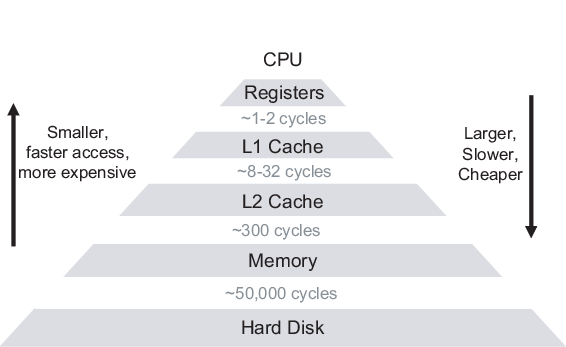
\includegraphics[width=0.6\textwidth]{figures/3_cpu/CPUherarchy.png}
	\caption{Hierarchy of memory types based on speed, cost, and capacity.}
\end{figure}

\subsubsection*{Cache Memory Operation}

% Explaining cache operation in detail
Cache memory operates on the principle of \textbf{locality}, which refers to the tendency of programs to access data and instructions that are close to each other in memory (spatial locality) or accessed repeatedly within a short time frame (temporal locality). The cache stores a subset of the main memory's contents in small, fast memory blocks called \textbf{cache lines}, typically 64 bytes in size. When the CPU requests data, the cache controller checks if the data resides in the cache. If it does (a \textbf{cache hit}), the data is retrieved quickly without accessing RAM. If it does not (a \textbf{cache miss}), the controller fetches the data from RAM or a lower-level cache, loading it into the cache for future access.

The cache is organized into \textbf{sets} and \textbf{ways}, forming an associative structure. For example, in a 4-way set-associative cache, each set can store four cache lines, and the cache controller uses a mapping function to determine which set a memory address corresponds to. If the target set is already full, the controller must evict a line (typically the least recently used) and repeated conflicts that keep evicting lines from the same set are known as \textbf{cache thrashing} \cite{CPUcachetrashing}.

\vspace{0.5em}

\begin{figure}[H]
	\centering
	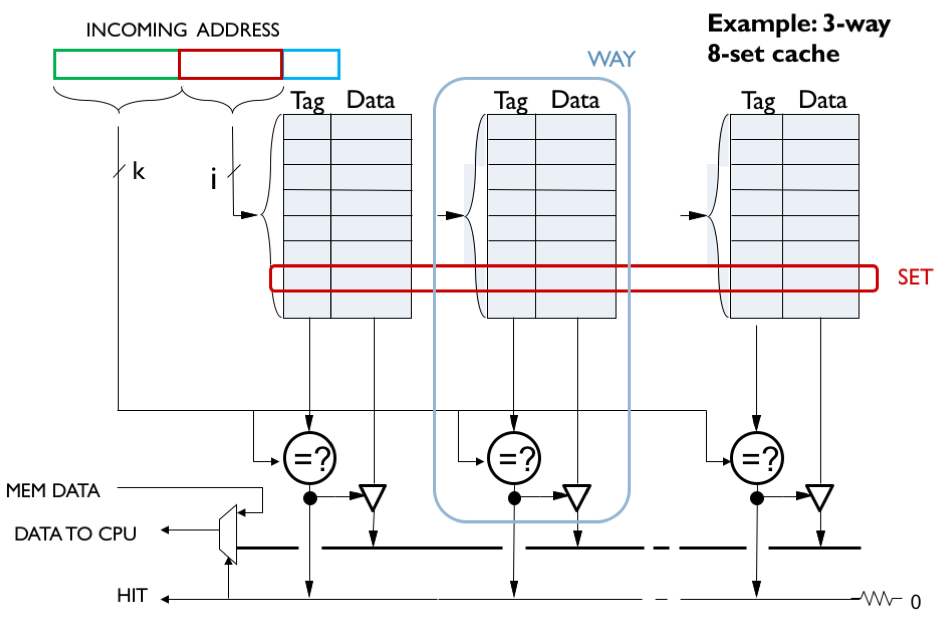
\includegraphics[width=0.75\textwidth]{figures/3_cpu/cache_ways_sets.png}
	\caption{\textbf{Set-associative cache (sets and ways).} Memory is cached in fixed-size lines (typically 64 B). When many cache addresses map to the same set and exceed the set's capacity, thrashing occurs. This organization explains why strided access patterns (e.g., row/column scans in matrices) can perform very differently depending on stride and problem size.}
\end{figure}

For now, we just need to understand the basic concepts of cache organization, including the roles of sets and ways, as well as the implications of cache hits and misses. But as we can see in the figure, this can be quite complex. Later sections will illustrate these concepts with practical examples.
\clearpage

\subsubsection*{RAM (Random Access Memory)}

\textbf{RAM} serves as the primary workspace for the CPU, storing data and program instructions that are actively in use. Unlike registers and cache, RAM offers significantly larger capacity (typically from 8GB to 64GB) but at the cost of much slower access speeds.

In an ideal scenario, the CPU retrieves the data it needs directly from its registers or from the cache, which are both extremely fast. However, if the required data is not present in any level of the cache hierarchy, a \textbf{cache miss} occurs. In this case, the CPU is forced to fetch the data from RAM, introducing a considerable delay in execution due to the higher memory latency.

This delay becomes particularly problematic in operations with low operation-to-data ratios, such as matrix-vector multiplication. As discussed in Chapter \ref{ch::chapter1}, Section\ref{subsec::operation_data_ratio}, MxV operations require frequent access to large portions of memory for relatively few computations, making them highly prone to cache misses. On the other hand, matrix-matrix multiplication (MxM) has a much higher operation-to-data ratio, allowing for better data reuse and more efficient use of the cache.

The performance of RAM is commonly described by two metrics: its \textbf{frequency} (in MHz), which affects memory bandwidth, and its \textbf{CAS latency} \cite{caslatency} (Column Access Strobe, or CL), which impacts memory access delay. CAS latency represents the number of clock cycles that elapse between the moment a memory controller sends a read command to a RAM module and when the data becomes available. However, since frequency determines how long each clock cycle lasts, the effective latency in nanoseconds is given by:

\[
\text{Latency (ns)} = \frac{\text{CL} \times 1000}{\text{Frequency (MHz)}}
\]

Hence, a higher frequency does not necessarily imply faster access unless CL is also considered. For instance, CL16 at 3200MHz results in a similar real latency to CL19 at 4000MHz:

\renewcommand{\arraystretch}{1.6}
\begin{table}[h!]
	\centering
	\begin{tabular}{|c|c|c|}
	\hline
	\textbf{Memory Speed} & \textbf{CAS Latency (CL)} & \textbf{Approx. Latency (ns)} \\ \hline
	3200 MHz             & CL16                      & $\frac{16 \times 1000}{3200} \approx 5$ ns \\ \hline
	4000 MHz             & CL19                      & $\frac{19 \times 1000}{4000} \approx 4.75$ ns \\ \hline
	2400 MHz             & CL17                      & $\frac{17 \times 1000}{2400} \approx 7.08$ ns \\ \hline
	\end{tabular}
	\caption{Estimated memory latency for different RAM configurations.}
\end{table}

Even newer memory technologies such as DDR5 aim to increase bandwidth and reduce latency through architectural improvements, such as dual or quad independent memory channels and higher burst lengths. However, the fundamental limitation of main memory remains: it is still significantly slower than L1, L2, or L3 cache, and orders of magnitude slower than registers.

\clearpage

\subsection{Cache Locality and Blocking}
\label{sec:cache_locality_and_blocking}

\textbf{Cache locality} refers to the efficient use of data elements that are either close together in memory (\textbf{spatial locality}) or accessed repeatedly in a short time frame (\textbf{temporal locality}). This aligns with how caches store data in 64-byte cache lines to minimize slower main memory access.

\textbf{Blocking} or tiling improves cache locality by dividing computations into smaller blocks that fit within cache, reducing cache misses and optimizing data reuse, especially beneficial for matrix multiplication. \cite{blocking}

In \textbf{Naive matrix multiplication}, each element $C(i,j)$ accesses entire row $A(i,*)$ and column $B(*,j)$. For large $N$, strided accesses (jumps of $N \times \text{element size}$ bytes) cause cache thrashing as data doesn't fit in cache and repeated accesses evict previously loaded cache lines.

\begin{figure}[H]
    \centering
    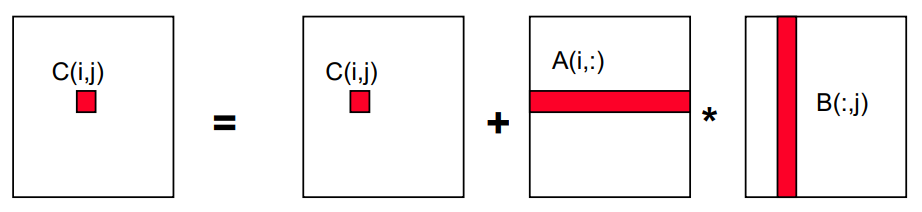
\includegraphics[width=0.9\textwidth]{figures/3_cpu/naiveMxM.png}
    \caption{Naive matrix multiplication algorithm.}
\end{figure}

\textbf{Blocked multiplication} partitions $A$, $B$, and $C$ into $b \times b$ blocks where $b$ fits in cache. For a 32KB L1 cache with FP32 elements, since three blocks must reside simultaneously:
\[
3b^2 \leq 8192 \quad \Rightarrow \quad b \leq \sqrt{\tfrac{8192}{3}} \approx 52
\]

The algorithm uses outer loops over blocks and inner loops for standard multiplication on each block, ensuring all necessary data resides in cache and leveraging both spatial and temporal locality.

\begin{figure}[H]
    \centering
    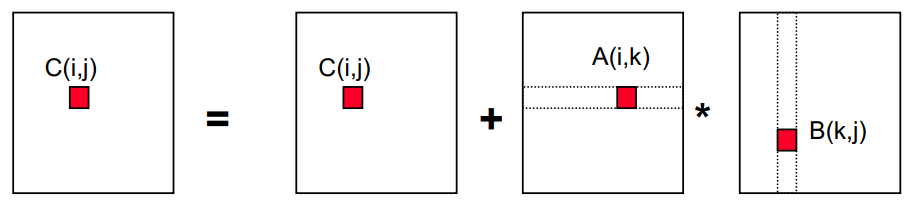
\includegraphics[width=0.9\textwidth]{figures/3_cpu/blockingMxM.png}
    \caption{Blocked matrix multiplication algorithm.}
\end{figure}

As mentioned in Chapter \ref{ch::chapter2}, blocking enables aggressive data reuse: tiles are reused $O(b)$ times, raising arithmetic intensity by factor $b$. Good blocking approaches the ideal $\tfrac{2}{3}N$ intensity, while naive approaches collapse to $O(1)$ due to repeated reloading. Libraries like BLAS and MKL implement these optimizations automatically.

\newpage

\section{Benchmarking on CPU}

In this section, we benchmark and compare the performance of \textbf{matrix–matrix multiplication} (MxM) and \textbf{matrix–vector multiplication} (MxV).  
The aim is to measure, for each operation, the sustained performance in $GFLOPS$ as the matrix size $N$ increases, and to contrast these measurements with theoretical limits imposed by both computation and memory access.

\vspace{0.5em}

\subsection*{Theoretical Compute Performance}

The theoretical time required to execute a given number of floating–point operations, assuming the CPU operates at its peak throughput, can be estimated as:
\begin{equation}
t_{CPU} = \frac{N_{ops}}{GFLOPS \times 10^9} \times 10^6,
\end{equation}

where $t_{CPU}$ is in microseconds. 

The peak performance in $GFLOPS$ is computed as:

\begin{equation}
GFLOPS = C_{CPU} \times CPU_{GHz} \times V_{vec} \times M_{ops}.
\end{equation}

\noindent The terms in the equation are:
\begin{itemize}
    \item $C_{CPU}$: number of \textbf{physical} CPU cores (logical threads are not counted here).
    \item $CPU_{GHz}$: CPU clock speed in GHz.
    \item $V_{vec}$: SIMD vector width in elements, which depends on the data type (e.g., single-precision 32-bit floats or double-precision 64-bit floats) and the instruction set architecture. The vector width $V_{vec}$ represents the number of elements that can be processed simultaneously in a single SIMD instruction. For example:
        \begin{itemize}
            \item Using \textbf{single-precision (F32, 32-bit)}:
                \begin{itemize}
                    \item AVX-512: $V_{vec} = 512 / 32 = 16$ elements per vector.
                    \item AVX2 (256-bit): $V_{vec} = 256 / 32 = 8$ elements per vector.
                \end{itemize}
            \item Using \textbf{double-precision (F64, 64-bit)}:
                \begin{itemize}
                    \item AVX-512: $V_{vec} = 512 / 64 = 8$ elements per vector.
                    \item AVX2 (256-bit): $V_{vec} = 256 / 64 = 4$ elements per vector.
                \end{itemize}
        \end{itemize}
    \item $M_{ops}$: floating–point operations per cycle per vector unit.
    For Fused Multiply–Add (FMA) \cite{FMA} instructions, each operation performs one multiplication and one addition in a single step, counting as two floating–point operations.
    For example, AVX2 \cite{AVX2} on the AMD Ryzen 5 5600X (Zen 3) can execute $2$ FMAs per cycle, resulting in $M_{ops} = 2 \times 2 = 4$.
\end{itemize}

\clearpage

\subsection*{Theoretical Memory Access Performance}

Even if the compute units can, in theory, reach a certain $GFLOPS$ peak, performance may be limited by memory bandwidth if it relies on it. This limitation arises because the rate at which data can be transferred to and from RAM often becomes a bottleneck, especially for memory-intensive operations such as matrix multiplications or large-scale vector computations. To estimate the time required to read or write the necessary data from/to RAM, we use a simplified model:

\begin{equation}
t_{mem} = \frac{N_{data}}{RAM_{Hz}} \times 10^6,
\end{equation}

where the terms are defined as follows:

\begin{itemize}
    \item $N_{data}$: the number of data elements that must be loaded from or stored into memory. This value depends on the specific operation being performed, such as the total number of elements in a matrix for matrix-matrix multiplication ($2 \cdot N^2$ for reading and writing) or the combined elements of a matrix and vector for matrix-vector multiplication ($N^2 + N$).
    \item $RAM_{Hz}$: the effective memory frequency in Hertz, which represents the clock rate at which the RAM operates. This frequency determines the maximum theoretical data transfer rate, assuming ideal conditions without overheads or inefficiencies.
\end{itemize}

This simplified model assumes that each clock cycle of the RAM can transfer one data element, and the time is converted to microseconds by multiplying by $10^6$.

However, it is important to note that this is a theoretical estimate and does not account for factors such as memory controller latency, bus contention, or the caches. For a more accurate estimation, one might consider the effective bandwidth and data size per element, but this model provides a baseline for understanding memory access costs.

For matrix-matrix multiplication (MxM), we estimate the real total memory access time by summing the individual measured components: the time to access a matrix by rows, the time to access a matrix by columns, and the time to allocate a matrix.

For matrix-vector multiplication (MxV), we sum the time to access a matrix by rows, the time to access a vector, and the time to allocate a vector.

\clearpage

\subsection{Benchmark Methodology}

The \textbf{GFLOPS benchmarks} are run using the \texttt{GFLOPS.jl} script where we do the following:
\begin{enumerate}
    \item Allocate:
    \begin{itemize}
        \item $A$: random $N \times N$ with \texttt{Float32} or \texttt{Float64} matrix.
        \item $B_{mat}$: random $N \times N$ with \texttt{Float32} or \texttt{Float64} matrix (for MxM).
        \item $B_{vec}$: random $N \times 1$ with \texttt{Float32} or \texttt{Float64} vector (for MxV).
    \end{itemize}
    \item Perform a \textbf{single multiplication} using \texttt{@benchmark} (\texttt{evals=1, samples=300}).
    \item Use the \textbf{minimum measured time} to approximate the sustained peak performance, reducing variability from noise and cache effects.
    \item Compute the sustained performance:
    \[
    GFLOPS_{\mathrm{MxM}} = \frac{2 N^3}{t_{MxM}} \times 10^{-9}, \quad
    GFLOPS_{\mathrm{MxV}} = \frac{2 N^2}{t_{MxV}} \times 10^{-9}.
    \]
\end{enumerate}

The \textbf{theoreticals memory access time $t_{mem}$ and compute time $t_{CPU}$ benchmarks} are run using the \texttt{tcpu\_tmemory.jl} and \texttt{tmemory.jl} scripts where we do the following:
\begin{enumerate}
    \item Compute the \textbf{theoretical times}:
    \begin{itemize}
        \item theoretical $t_{CPU}$: using the total number of floating-point operations for MxM or MxV, the peak $GFLOPS$ reported by \texttt{cpu\_info()} and the number of physical cores. To provide a realistic estimate, we utilize the base clock frequency rather than the turbo boost frequency.
        \item theoretical $t_{mem}$: using the number of data elements and the RAM frequency.
    \end{itemize}
    \item Measure the \textbf{measured execution times} for:
    \begin{itemize} % quiero poner aquí las llamadas de benchmark, ;a sí que no se repite el código
        \item measured $t_{CPU}$: using \texttt{@benchmark} on the matrix-matrix multiplication of $A$ and $B_{mat}$ and on the matrix-vector multiplication of $A$ and $B_{vec}$.
        \item measured $t_{mem}$: using \texttt{@benchmark} on the memory access patterns of the matrices and vectors. Includes row-wise and column-wise accesses, as well as vector accesses.
    \end{itemize}
\end{enumerate}

\vspace{1em}

\subsubsection*{Libraries and System (CPU, RAM)}

All benchmarks and plots are using MKL \cite{MKL} (BLAS/LAPACK) library. OpenBLAS was also tested but generally performed worse, especially for small matrices with MxM multi-core. 

The host system is an AMD Ryzen 5 5600X \cite{Ryzen5600Xspecs} (6C/12T) with a 3.7\,GHz base frequency (this base clock is used for the theoretical GFLOPS estimate) and 32\,GB DDR4 memory running at 3200\,MHz.


\clearpage

\subsection{Benchmark results: GFLOPS}
\label{sec:cpu_bench_results_GFLOPS}

This section reports CPU GFLOPS for dense matrix kernels and organizes the discussion around five ideas:
(A) single-core MxM vs.\ MxV, (B) multi-core MxM vs.\ MxV, (C) single \& multi MxM vs.\ theoretical peaks, (D) low-$N$ behavior (overheads vs.\ asymptotics), and (E) an overview for Float64.

In brief: on a single core, MxM consistently outperforms MxV; with multiple cores, MxM benefits markedly from parallelism while MxV remains bandwidth-bound; the single-core MxM curve tracks its theoretical limit closely, whereas the multi-core curve remains below its ideal due to shared-resource contention; at small sizes, parallel overheads can outweigh benefits; and Float64 sustains lower throughput but preserves the same qualitative behavior.

\subsubsection*{(A) FP32: Single-core \textnormal{MxM} vs.\ \textnormal{MxV}}
On a single core, matrix--matrix multiplication (MxM) delivers substantially higher GFLOPS than matrix--vector (MxV) across sizes. MxM is compute-bound with high arithmetic intensity ($O(N^3)$ work over $O(N^2)$ data), letting BLAS microkernels keep FMA pipelines busy and reuse cache-blocked tiles effectively. By contrast, MxV performs much less work per byte moved ($O(N^2)$ work over $O(N^2)$ data), so performance is limited by memory bandwidth and remains relatively flat with~$N$.

\begin{figure}[H]\centering
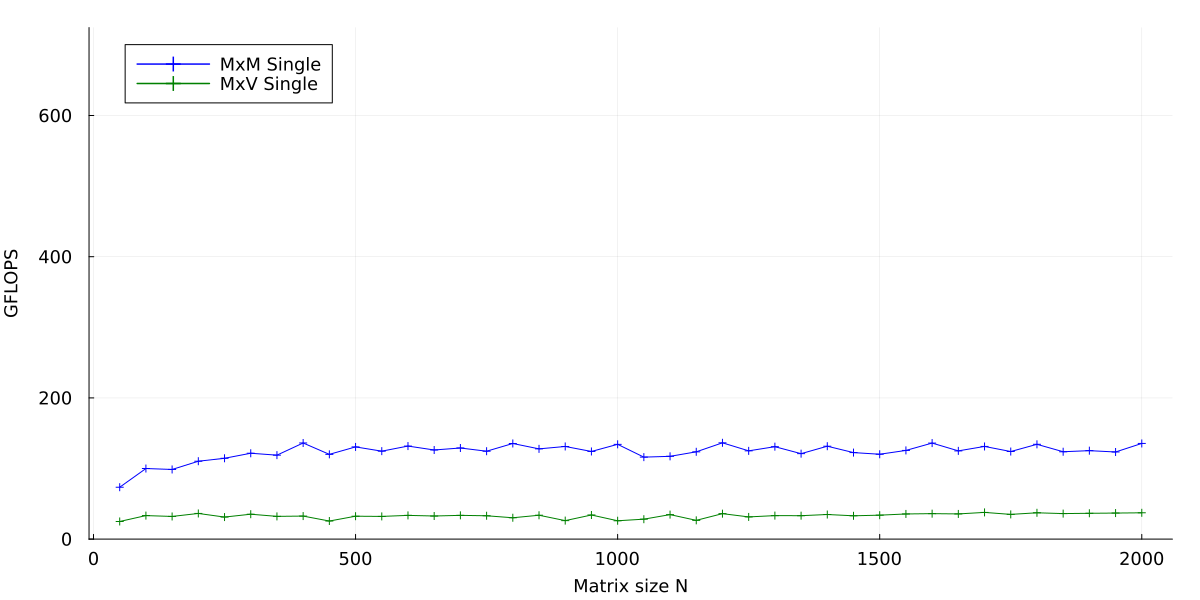
\includegraphics[width=\textwidth]{figures/3_cpu/gflops/Float32_GFLOPS_Ryzen5_5600X_MxM_vs_MxV_Single.png}
\caption{\textbf{FP32, single-core: MxM vs.\ MxV.} MxM clearly outperforms MxV across sizes. The reason is arithmetic intensity: MxM amortizes memory traffic via cache-blocked tiles and sustains high utilization of FMA units (compute-bound), whereas MxV quickly becomes limited by memory bandwidth (memory-bound), yielding a flatter, lower curve.}
\label{fig:cpu_gflops_fp32_single_mxm_mxv}
\end{figure}

\subsubsection*{(B) FP32: Multi-core \textnormal{MxM} vs.\ \textnormal{MxV}}
With multiple cores, MxM benefits strongly once $N$ is large enough for effective parallelism: the workload exposes ample independent blocks, and threading overheads become negligible relative to the total compute.

In contrast, MxV exhibits little separation between single-core and multi-core curves because additional cores share the same memory subsystem, so bandwidth remains the bottleneck.

\begin{figure}[H]\centering
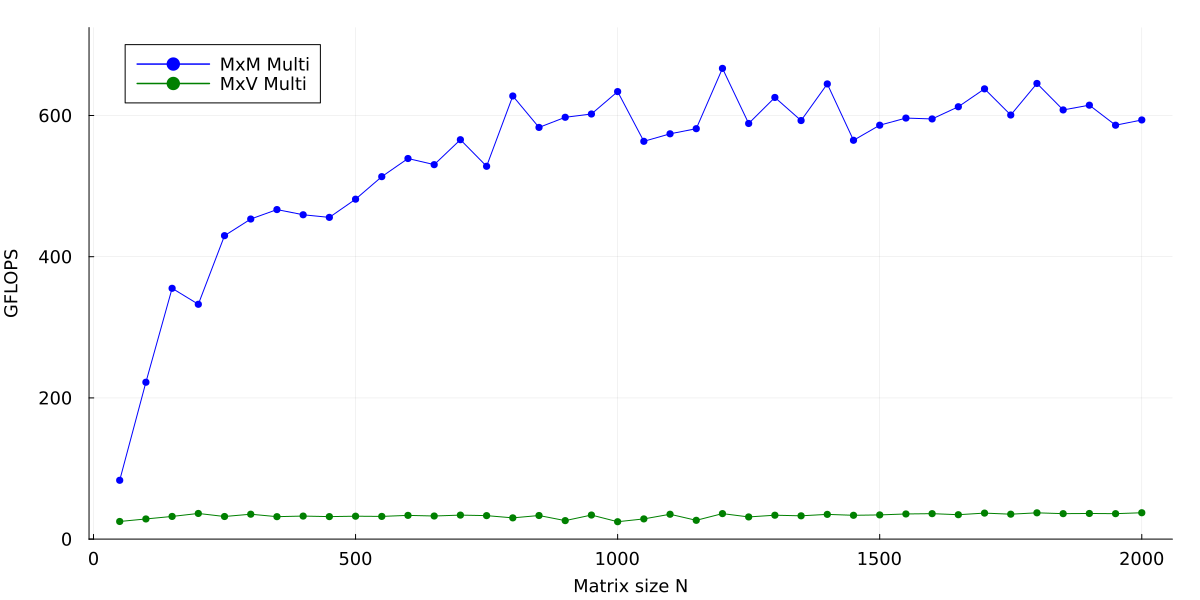
\includegraphics[width=\textwidth]{figures/3_cpu/gflops/Float32_GFLOPS_Ryzen5_5600X_MxM_vs_MxV_Multi.png}
\caption{\textbf{FP32, multi-core: MxM vs.\ MxV.} MxM gains markedly from parallelism once $N$ is sufficient to amortize threading overheads and feed all cores; MxV barely scales because RAM bandwidth is shared and already constraining performance, so extra cores cannot increase sustained FLOPS meaningfully.}
\label{fig:cpu_gflops_fp32_multi_mxm_mxv}
\end{figure}

Something to mention is that we see a slight drop for the largest $N$ near the end of the benchmark in MxM.

This behavior is typical under sustained all-core load: (i) power/thermal limits reduce all-core turbo frequencies (thermal or power throttling), and (ii) the working set exceeds the last-level cache, pushing more traffic to RAM because of cache misses.

\clearpage

\subsubsection*{(C) FP32: \textnormal{MxM} (single \& multi) vs.\ theoretical}
Comparing measured MxM to theoretical ceilings clarifies limits. The single-core curve typically tracks its peak closely because there is no inter-core contention and BLAS microkernels keep pipelines saturated with regular access patterns.

The multi-core curve, however, stays below its ideal due to lower all-core frequencies mostly because of power/thermal constraints, shared last-level cache and memory bandwidth.

\begin{figure}[H]\centering
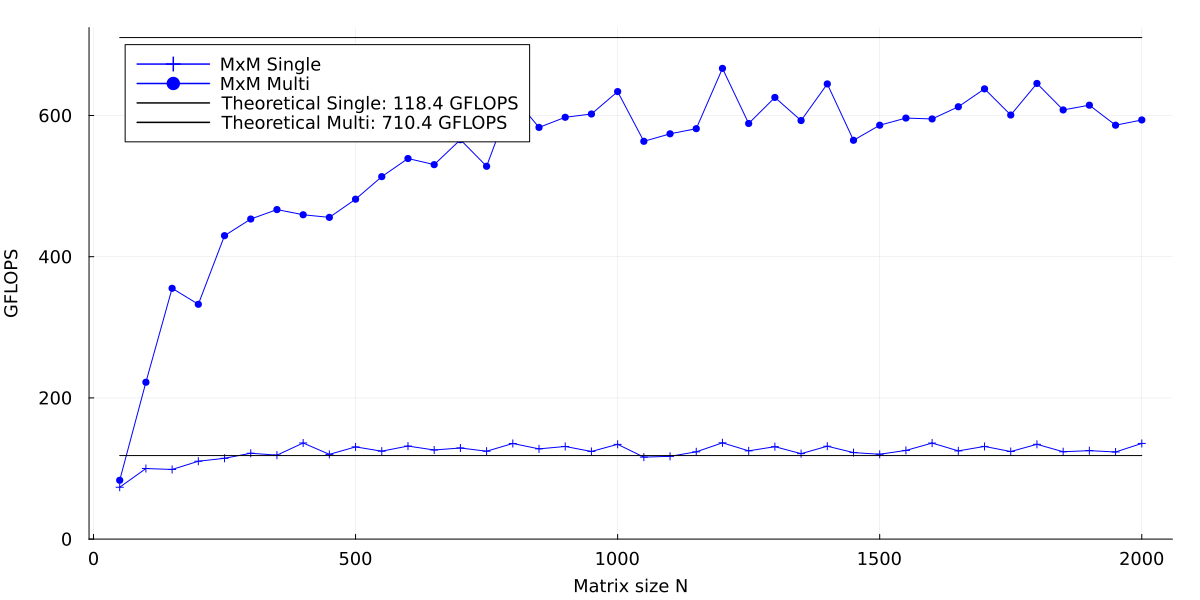
\includegraphics[width=\textwidth]{figures/3_cpu/gflops/Float32_GFLOPS_Ryzen5_5600X_MxM_Theo.png}
\caption{\textbf{FP32: MxM (single \& multi) vs.\ theoretical.} Single-core MxM exceeds the theoretical line thanks to efficient microkernel execution and no resource contention. Multi-core MxM rises with $N$ but remains below its theoretical bound because all-core turbo is lower than single-core boost and shared resources (shared L3 cache, memory bandwidth) and coordination overheads limit scaling.}
\label{fig:cpu_gflops_fp32_mxm_theoretical}
\end{figure}

It is important to note that the theoretical GFLOPS have been calculated by the script \texttt{system\_info.jl}, for the Ryzen 5 5600X, using the \textbf{base clock speed} and the number of cores. This is why the theoretical values are lower than the measured values in single core as they do not account for the boost clock speeds that are utilized during benchmarking when only a single core is active.

\clearpage

\subsubsection*{(D) FP32: Low-$N$ behavior (zoom)}
At small sizes, parallelization costs dominate: thread creation, synchronization, and less effective cache blocking can make multi-core performance match or even trail single-core. Those constant-time costs that are not negligible as at large $N$.

As $N$ grows, the asymptotic $O(N^3)$ compute of MxM quickly overwhelms overheads, tiles fit better into the blocking strategy, and multi-core scaling emerges toward its plateau.
\begin{figure}[H]\centering
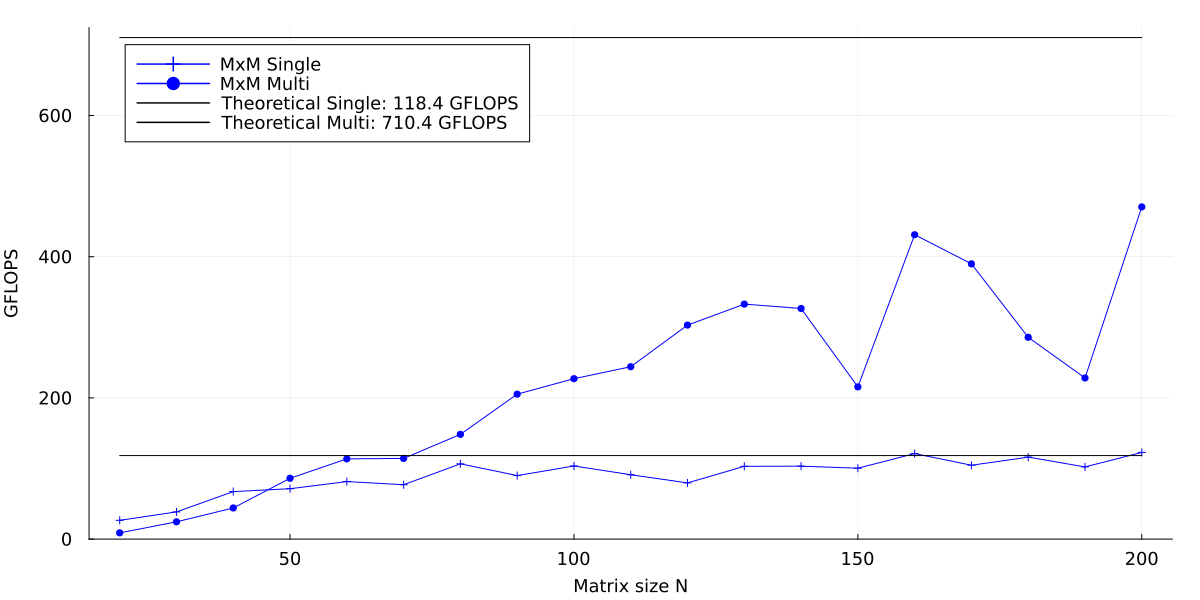
\includegraphics[width=\textwidth]{figures/3_cpu/gflops/Float32_GFLOPS_Ryzen5_5600X_MxM_Theo_lowN.png}
\caption{\textbf{FP32 (low-$N$ zoom): single vs.\ multi vs.\ theoretical for MxM.} For tiny matrices, multi-core can underperform due to overheads and limited reuse; single-core often benefits from excellent locality. Increasing $N$ restores the expected order: multi-core overtakes single-core as blocking becomes effective and parallel work dwarfs coordination costs.}
\label{fig:cpu_gflops_fp32_mxm_theoretical_lown}
\end{figure}

In practice, optimized libraries like MKL often employ dynamic threading (using few threads for small $N$, then increasing) precisely to avoid oversubscription in this regime, but this would not be as effective as using a single thread for very small $N$.


\clearpage

\subsubsection*{(E) Float64 (overview)}
With Float64, throughput drops relative to Float32 while preserving the same qualitative picture: MxM remains compute-bound and benefits from larger $N$ and multi-core parallelism, whereas MxV stays bandwidth-bound with minimal scaling.

The gap to multi-core theoretical peaks tends to widen because doubling the data size increases cache pressure and effective bandwidth demands per operation, accentuating shared-resource limits.

\begin{figure}[H]\centering
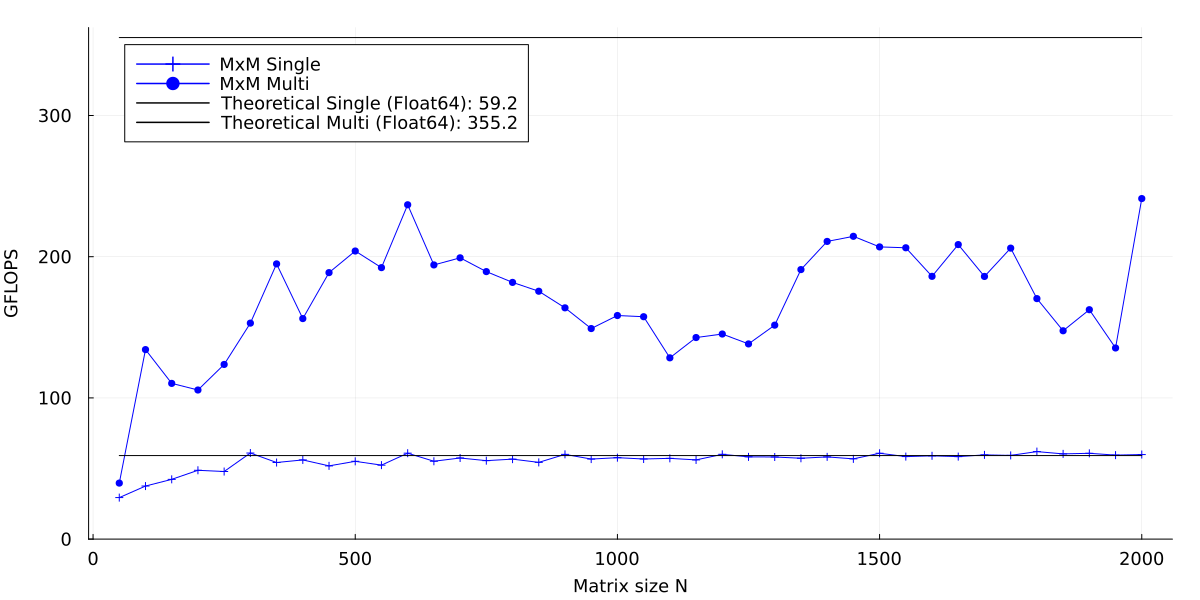
\includegraphics[width=\textwidth]{figures/3_cpu/gflops/Float64_GFLOPS_Ryzen5_5600X_MxM_Theo.png}
\caption{\textbf{FP64: MxM (single \& multi) vs.\ theoretical.} Same trends as FP32 with lower absolute throughput and a larger gap to the multi-core theoretical due to SIMD/FMA processing half as many elements per cycle and doubles consume twice the bytes and due to higher memory pressure and shared-resource contention}
\label{fig:cpu_gflops_fp64_mxm_theoretical}
\end{figure}

\textbf{y-axis scale warning:} When comparing FP64 and FP32 plots, be careful with the y-axis scale: FP64 theoretical peaks are roughly half of FP32 because a fixed-width SIMD register (e.g., AVX2 at 256 bits) holds half as many elements (4 doubles vs.\ 8 floats), halving FMA throughput per cycle. Additionally, as we already said, each element is twice the size, increasing memory pressure for bandwidth-bound kernels.


\clearpage

\subsection{Benchmark results: theoretical vs measured time}
\label{sec:cpu_bench_results_theoretical_vs_measured_time}

This section compares theoretical compute time ($t_{\text{CPU}}$) and theoretical memory time ($t_{\text{mem}}$) against measured execution times for MxM and MxV operations in a multi-core context.

The theoretical curves act as lower bounds: $t_{\text{CPU}}$ assumes perfect peak FLOPS utilization without stalls, while $t_{\text{mem}}$ assumes RAM-limited access without cache hierarchy benefits or overheads. Measured curves include those real effects.

\subsubsection*{(A) FP32: $t_{\text{CPU}}$ vs.\ $t_{\text{mem}}$ \textnormal{in MxM}}
For MxM, the operation-to-data ratio dominates the shape: the useful work grows as $O(N^3)$ while the moved data is $O(N^2)$. Consequently, $t_{\text{CPU}}$ grows faster with $N$ than $t_{\text{mem}}$. Optimized BLAS kernels (blocking/tiling) maximize reuse so the measured time follows the compute-bound trend and stays well above $t_{\text{mem}}$ for moderate and large $N$.

\begin{figure}[H]\centering
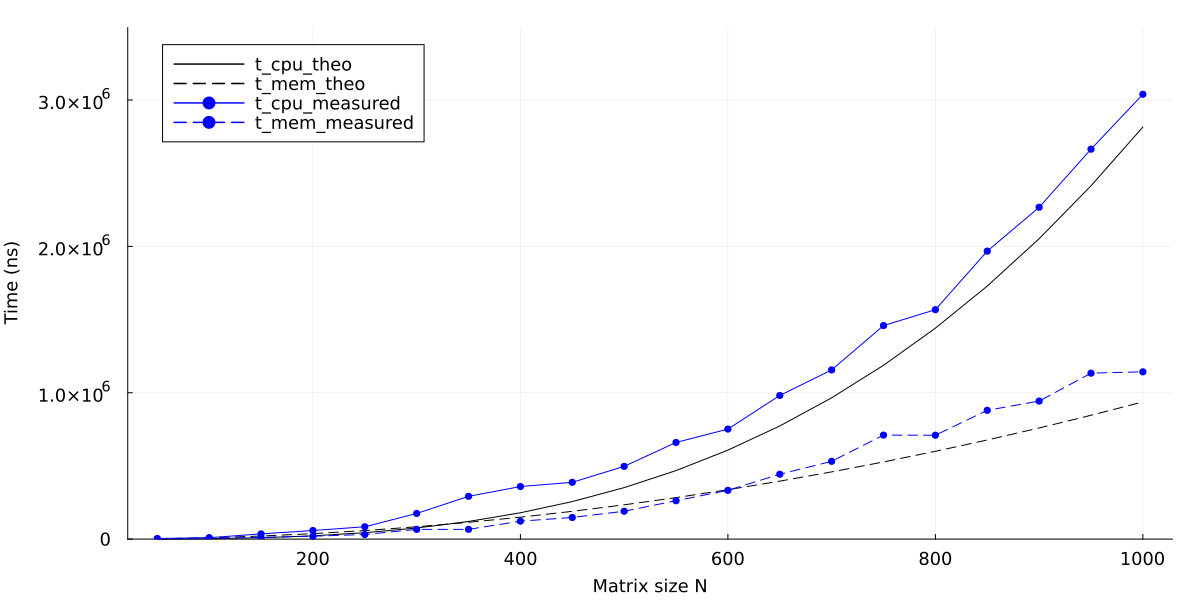
\includegraphics[width=\textwidth]{figures/3_cpu/tcpu_tmemory/Float32_MXM_Ryzen5_5600X.png}
\caption{\textbf{FP32 MxM: theoretical vs.\ measured times.} $t_{\text{CPU}}$ scales as $O(N^3)$ and dominates for moderate/large $N$; measured time tracks the compute-bound model thanks to cache-blocked reuse. $t_{\text{mem}}$ is a lower bound assuming RAM-limited traffic; real runs reuse data from caches and remain above it.}
\label{fig:tcpu_tmem_mxm_f32_full}
\end{figure}

Measured $t_{\text{mem}}$ is below the theoretical line across small and mid sizes (consistent with L1/L2/L3 reuse). A gentle crossover where measured $t_{\text{mem}}$ overtakes the RAM-only bound appears only near the upper end of the tested $N$ range, matching the expectation that cache capacity and controller saturation effects surface late in MxM due to strong reuse.

\clearpage

\subsubsection*{(B) FP32: $t_{\text{CPU}}$ vs.\ $t_{\text{mem}}$ \textnormal{in MxV}}
MxV has low arithmetic intensity ($O(N^2)$ FLOPs over $O(N^2)$ data) and quickly becomes bandwidth-bound. Here the theoretical $t_{\text{mem}}$ tends to dominate $t_{\text{CPU}}$.

For large $N$, the  memory time exceeds the theoretical bound due to cache misses, row/column conflict patterns and contention in the memory controller, none of which are modeled in the simple $t_{\text{mem}}$ bound.

\begin{figure}[H]\centering
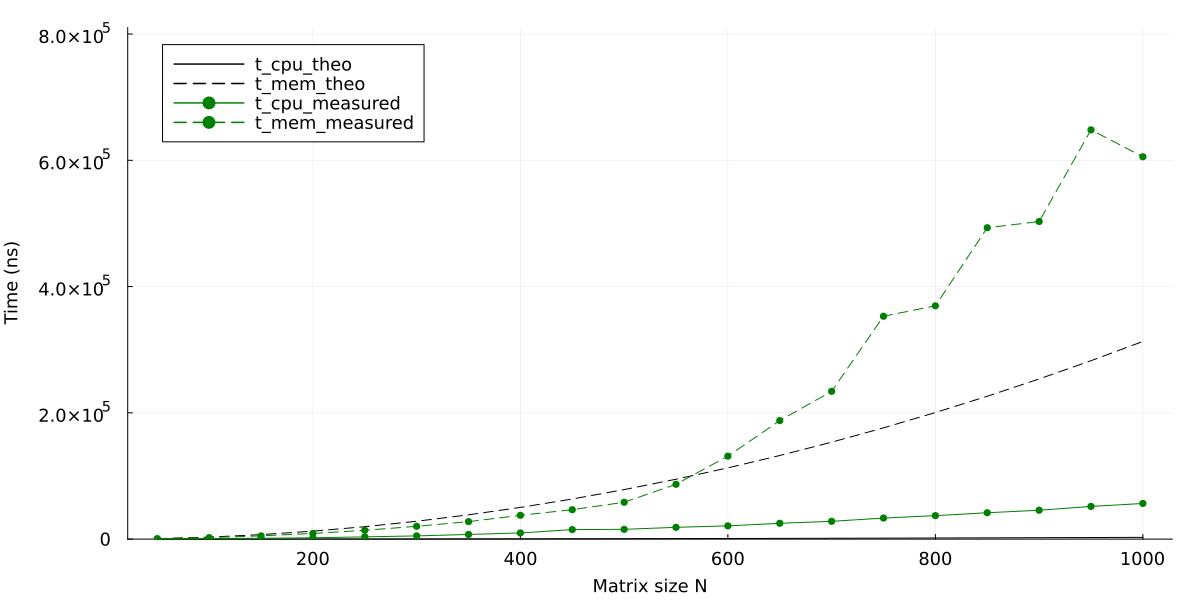
\includegraphics[width=\textwidth]{figures/3_cpu/tcpu_tmemory/Float32_MXV_Ryzen5_5600X.png}
\caption{\textbf{FP32 MxV: theoretical vs.\ measured times.} Bandwidth-bound across sizes: $t_{\text{mem}}$ dominates $t_{\text{CPU}}$. At large $N$, the measured memory time rises above the theoretical curve due to cache misses and controller saturation not captured by the simple RAM-bound model.}
\label{fig:tcpu_tmem_mxv_f32_full}
\end{figure}

The divergence (measured $t_{\text{mem}}$ climbing above the RAM-only line) appears already at mid-to-large sizes, earlier than in MxM and climbing faster due to the lower reuse in GEMV, which leads to increased memory pressure and contention. Keep in mind that the RAM-only bound is a simplified model that doesn't account for these overheads, causing the measured performance to be worse than predicted when cache efficiency degrades and memory subsystem bottlenecks emerge.

\clearpage

\subsubsection*{(C) FP32 (low-$N$ zoom): $t_{\text{CPU}}$ vs.\ $t_{\text{mem}}$ \textnormal{in MxM}}
With low-$N$, we see that the measured $t_{\text{CPU}}$ curve sits goes above what we expect, this is because of coordination costs multi-core overheads and short-run effects.

This can place the measured $t_{\text{CPU}}$ curve above the measured $t_{\text{mem}}$ initially, something that is maybe counterintuitive if we think that in these low-$N$ regimes, the impact of cache usage would help where all data fits in cache.

Those overheads can also be spotted in very low $N$ in the measured $t_{\text{mem}}$ curve, which can exceed the theoretical $t_{\text{mem}}$, because cache advantage does not overcome the increased coordination costs and multi-core overheads.

\begin{figure}[H]\centering
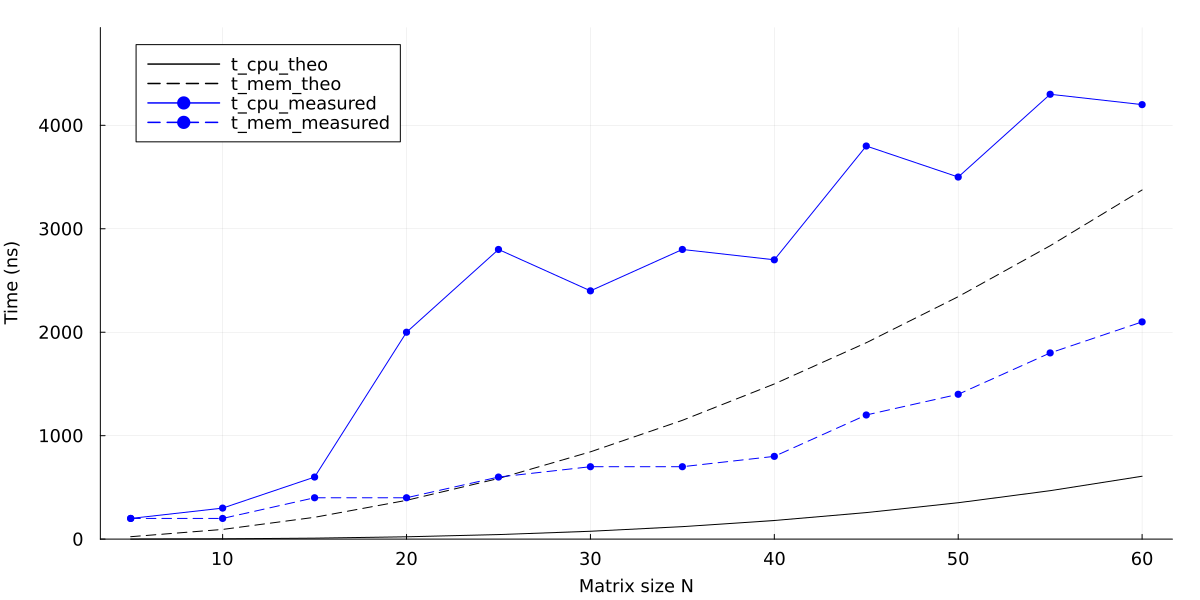
\includegraphics[width=\textwidth]{figures/3_cpu/tcpu_tmemory/Float32_MXM_Ryzen5_5600X_lowN.png}
\caption{\textbf{FP32 MxM (low-$N$ zoom):} In the low-$N$ regime, overheads can make measured $t_{\text{mem}}$ exceed the simple theoretical RAM-bound. The $t_{\text{CPU}}$ curve remains dominant as $N$ increases, reflecting the strong compute-bound nature of the operation.}
\label{fig:f32_mxm_60}
\end{figure}

Also, do not be misled if the theoretical $t_{\text{mem}}$ curve appears above the theoretical $t_{\text{CPU}}$ curve at tiny $N$ as the models scale differently. The theoretical $t_{\text{mem}}$ is quadratic in $N$ (e.g., $\sim 3N^2$ terms) while the theoretical $t_{\text{CPU}}$ is cubic (e.g., $\sim 2N^3$). For very small $N$, the quadratic with a larger constant sits above the cubic but as $N$ grows, the $N^3$ term inevitably dominates.

\clearpage

\subsubsection*{(D) \& (E) FP64: $t_{\text{CPU}}$ vs.\ $t_{\text{mem}}$ \textnormal{in MxM and MxV}}
In Float64, trends mirror FP32 but with larger data per element. Doubled bytes increase cache pressure and bandwidth demand, reflected in the $N$ at which measured $t_{\text{mem}}$ rises above the theoretical bound shifts to smaller sizes, reflecting earlier cache overflow.

\begin{figure}[H]\centering
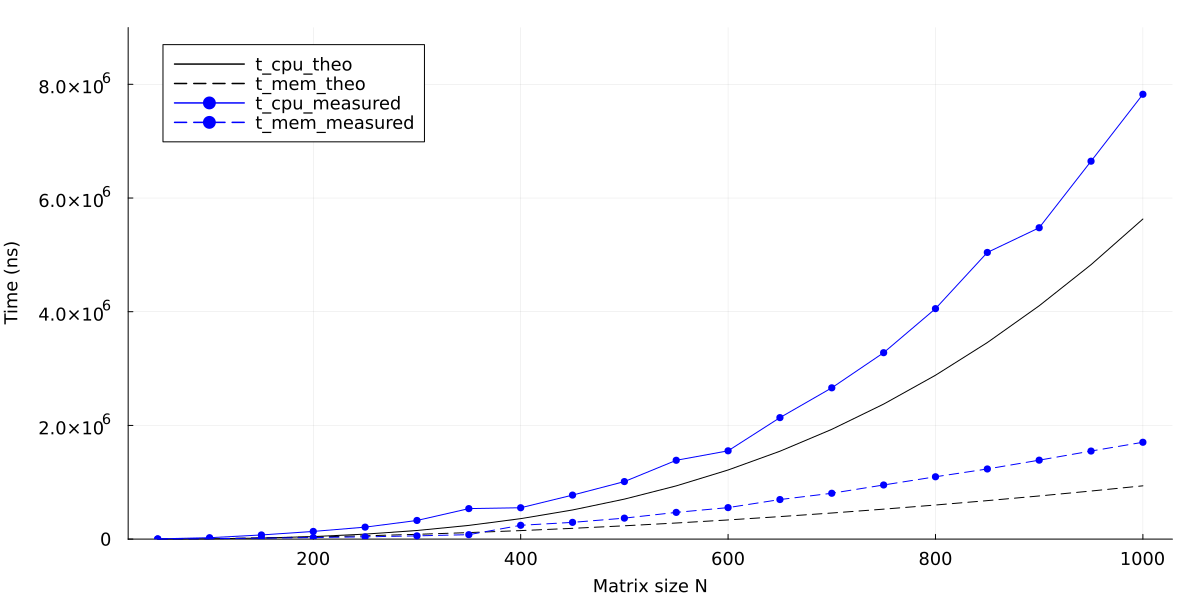
\includegraphics[width=\textwidth]{figures/3_cpu/tcpu_tmemory/Float64_MXM_Ryzen5_5600X.png}
\caption{\textbf{FP64 MxM: theoretical vs.\ measured times.} Same qualitative picture as FP32: compute-bound with measured times tracking $t_{\text{CPU}}$.}
\label{fig:tcpu_tmem_mxm_f64_full}
\end{figure}

\vspace{-1.5em}

\begin{figure}[H]\centering
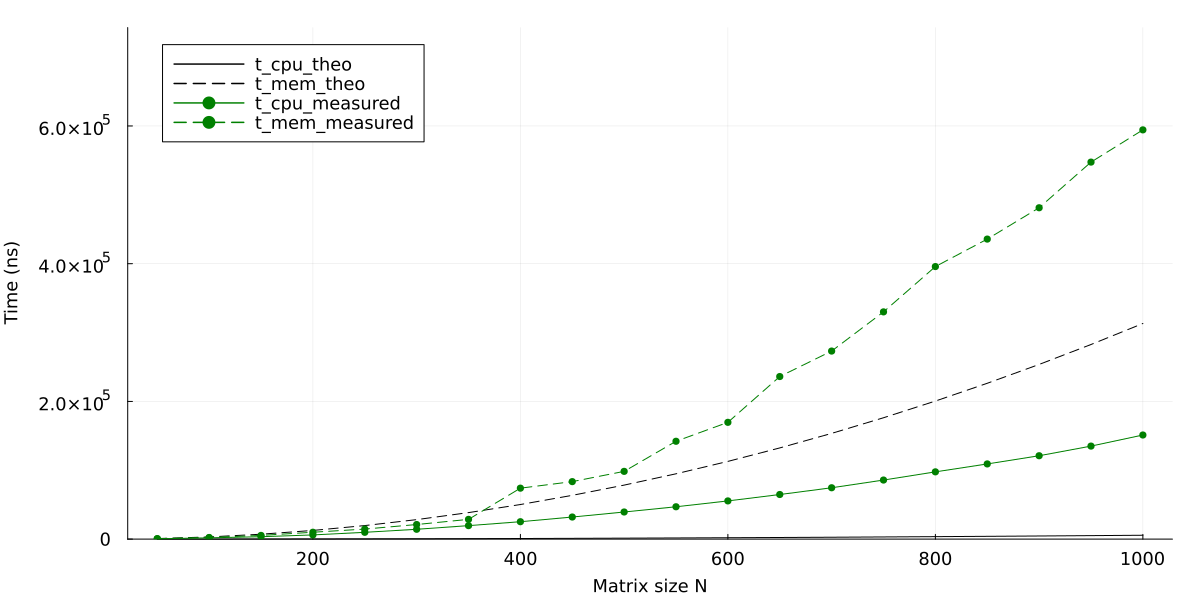
\includegraphics[width=\textwidth]{figures/3_cpu/tcpu_tmemory/Float64_MXV_Ryzen5_5600X.png}
\caption{\textbf{FP64 MxV: theoretical vs.\ measured times.} Even more bandwidth-bound than FP32: the crossover to measured $t_{\text{mem}}$ exceeding the theoretical bound occurs at smaller $N$ due to doubled element size and earlier cache overflow.}
\label{fig:tcpu_tmem_mxv_f64_full}
\end{figure}

\clearpage

\subsection{Benchmark results: cache conflict spikes}
\label{sec:cpu_bench_results_memory_conflict_spikes}

To expose cache–set conflicts explicitly, we rerun the memory-time experiment for \textbf{MxM} with a fine-grained grid of sizes \(N\) (step 8). We plot again the measured memory time for the kernel: the goal is to reveal conflict-driven spikes that can be masked by coarse sampling.

\subsubsection*{(A) FP32: conflict spikes with fine \(N\)}
In FP32, the memory-time curve shows pronounced spikes at regularly spaced sizes when scanning rows. In column-major layout, row-wise traversal advances by a stride of \(s=N\cdot \mathrm{sizeof}(\text{Float32})=4N\) bytes. With an L1 data cache of \(\,32\,\mathrm{KB}\), \(64\) sets, \(8\)-way associativity and \(64\)-byte lines, the set index advances by
\[
k \;=\; \frac{s}{64} \;=\; \frac{N}{16}\,.
\]
When \(k\) shares a large divisor with the \(64\) sets (e.g., \(N\) a multiple of \(128\)), accesses concentrate on few sets and saturate the \(8\)-way associativity, causing conflict misses and sharp latency spikes. Using a finer \(N\)-grid makes these resonances stand out clearly.

\begin{figure}[H]\centering
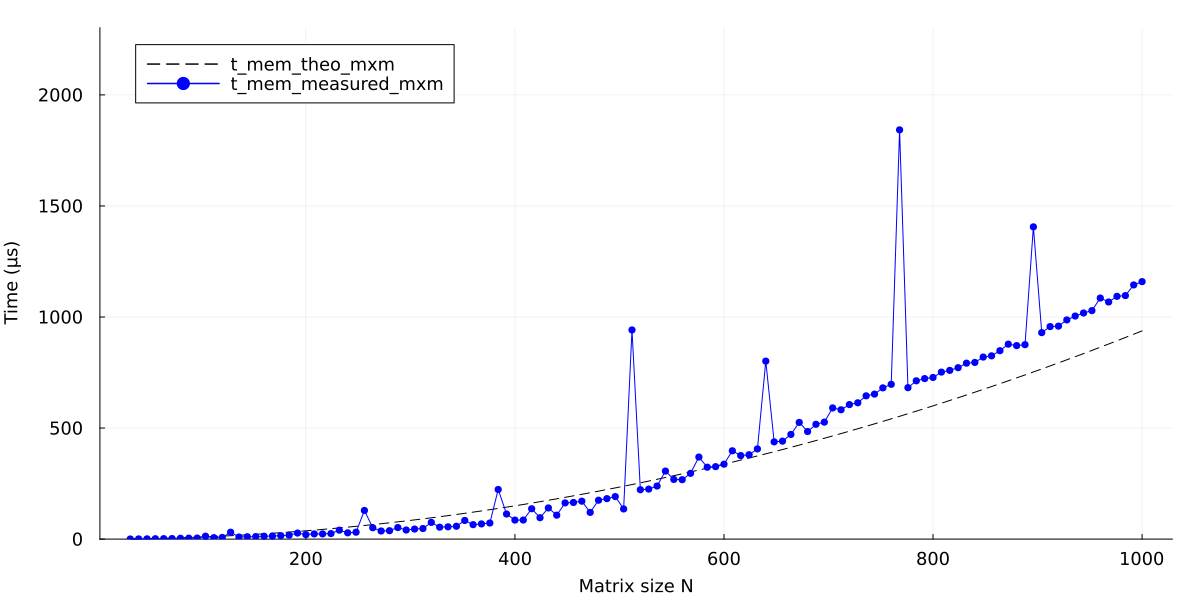
\includegraphics[width=0.95\textwidth]{figures/3_cpu/tmemory/Float32_MEMORY_MxM_Ryzen5_5600X.png}
\caption{\textbf{FP32 MxM (memory time, fine \(N\)).} Distinct spikes appear at conflict sizes where the row stride \(4N\) bytes aliases onto a small subset of the \(\,64\) L1 sets (32\,KB, 8-way, 64B lines). In those cases the set footprint exceeds the 8-way capacity and lines evict each other aggressively, inflating the measured memory time.}
\label{fig:mem_spikes_fp32}
\end{figure}

\vspace{-1em}

To understand the conflict spikes in an easier way, consider the following:

At \(N=128\), \(4N=512=64\times 8\): each column hop moves the cache set by exactly \(+8\), so you keep accessing the same 8 of 64 sets and overflow the 8-way associativity → spike.

At \(N=129\), \(4N=516=64\times 8+4\): that extra 4 bytes accumulates, so over time you visit all 64 sets and spread the pressure → no spike.

\clearpage

\subsubsection*{(B) FP64: same spikes plus interleaved ones}
In FP64, the same conflict sizes reappear and additional spikes emerge between them. The stride doubles to \(s=N\cdot \mathrm{sizeof}(\text{Float64})=8N\) bytes, so the set-step is
\[
k \;=\; \frac{s}{64} \;=\; \frac{N}{8}\,,
\]
which makes many more \(N\) satisfy the same aliasing condition (large \(\gcd(k,64)\)). As a result, conflict resonances occur more frequently (e.g., at multiples of \(64\), not only of \(128\)), producing interleaved spikes between the FP32 peaks. Moreover, each 64B line holds half as many elements (8 vs.\ 16), increasing pressure and amplifying spike height.

\begin{figure}[H]\centering
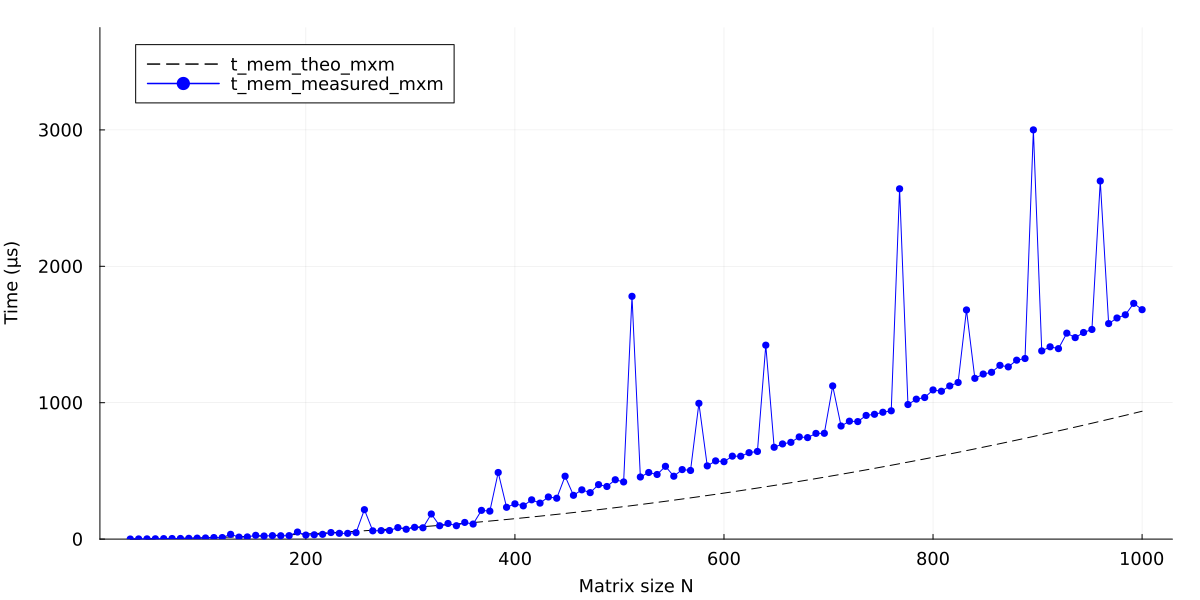
\includegraphics[width=0.95\textwidth]{figures/3_cpu/tmemory/Float64_MEMORY_MxM_Ryzen5_5600X.png}
\caption{\textbf{FP64 MxM (memory time, fine \(N\)).} The FP32 resonance sizes persist, and new interleaved spikes appear because the larger stride \(8N\) bytes increases the number of \(N\) that map onto few L1 sets (32\,KB, 64 sets, 8-way, 64B lines). With fewer doubles per line, conflict pressure is stronger and peaks are typically more pronounced.}
\label{fig:mem_spikes_fp64}
\end{figure}


